\begin{frame}
    \centering
    \begin{figure}[H]
        
\includegraphics[keepaspectratio, width=0.7\paperwidth, height=\paperheight]{LeeLogo}
    \end{figure}
    Informatik: Programmieren\\
    \emoji{cook} Kapitel 7: \textbf{Funktionen und \tjinline{return}}
\end{frame}
\fboxsep=.6pt
% default settings for listings
\lstset{style=TigerJython, basicstyle=\scriptsize\ttfamily,escapeinside={(*@}{@*)}}

\begin{frame}[fragile]{Funktionen}{Ein einfaches Beispiel}
\begin{lstlisting}
def summiere(x1, x2):
	summe = x1 + x2
	return summe
	
res = summiere(3,5)
print(res)
\end{lstlisting}

\end{frame}

\begin{frame}[fragile]{Funktionen}{Beispiel mit Turtle \emoji{turtle}}
\begin{minipage}{.7\textwidth}
\begin{lstlisting}
from gturtle import *
makeTurtle()
hideTurtle()

def vieleck(umfang, ecken):
    repeat ecken:
        fd(umfang/ecken)
        rt(360/ecken)

def vieleck_muster(umfang, ecken):
	(*@\only<2->{\colorbox{CornflowerBlue}{gesamtdistanz=0}}@*)
    while umfang>50:
        vieleck(umfang, ecken)
        (*@\only<3->{\colorbox{CornflowerBlue}{gesamtdistanz+=umfang}}@*)
        umfang-=10
        rt(10)
    (*@\only<4->{\colorbox{CornflowerBlue}{return gesamtdistanz}}@*)
    
(*@\only<5->{\colorbox{CornflowerBlue}{gesamtdistanz = }}@*)vieleck_muster(500,35)
(*@\only<6->{\colorbox{CornflowerBlue}{print(gesamtdistanz)}}@*)
\end{lstlisting}
% Clean code
%from gturtle import * 
%makeTurtle() 
%hideTurtle()
%gesamtdistanz=0
%def vieleck(umfang, ecken): 
%    repeat ecken:
%        fd(umfang/ecken)
%        rt(360/ecken)
%
%def vieleck_muster(umfang, ecken , gesamtdistanz ):
%    while umfang>50: 
%        vieleck(umfang, ecken)
%        gesamtdistanz+=umfang
%        umfang-=10 
%        rt(10)
%    return gesamtdistanz
%
%gesamtdistanz = vieleck_muster(500,35 , gesamtdistanz )

\end{minipage}
\begin{minipage}{.25\textwidth}
\begin{figure}[H]
	\centering
    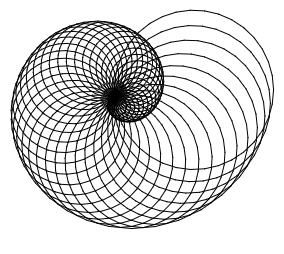
\includegraphics[keepaspectratio, width=\textwidth]{GrundlagenInfo/00_Programmieren/Figures/spirale.png}
\end{figure}

\end{minipage}
\end{frame}


\begin{frame}[fragile]{\tjinline{return}: Analogie \emoji{cook}}
Funktionen $\simeq$ Kochrezepte

\begin{lstlisting}
def gericht(zutat1, zutat2, zutat3):
    gericht = zutat1 + zutat2 + zutat3
    return (*@\only<1>{gericht}\only<2>{\colorbox{CornflowerBlue}{gericht}}@*)

# Beispiel 1 (funktioniert nicht! Nur zur Illustration)
(*@\only<1>{gericht}\only<2>{\colorbox{CornflowerBlue}{gericht}}@*) = gericht((*@ \tiny\emoji{bread}, \emoji{poultry-leg},\tiny \emoji{cheese} @*))
print(gericht) # (*@ \tiny\emoji{hamburger} @*)

# Beispiel 2 (funktioniert nicht! Nur zur Illustration)
(*@\only<1>{gericht}\only<2>{\colorbox{CornflowerBlue}{gericht}}@*) = gericht((*@ \tiny\emoji{tropical-fish}, \emoji{cooked-rice}, \emoji{salt} @*))
print(gericht) # (*@ \tiny\emoji{sushi} @*)

# Beispiel 3    
(*@\only<1>{gericht}\only<2>{\colorbox{CornflowerBlue}{gericht}}@*) = gericht(1, 5, 3)
print(gericht) # 9
\end{lstlisting}
\end{frame}

\begin{frame}[fragile]{Funktionen: Beispiel 2}
\begin{lstlisting}
def berechne_rechteck_flaeche((*@\only<1>{laenge, breite}\only<2->{\colorbox{CarnationPink}{laenge, breite}}@*)):
    flaeche = laenge * breite
    return (*@\only<1-2>{flaeche}\only<3->{\colorbox{CornflowerBlue}{flaeche}}@*)

def ist_grosse_flaeche((*@\only<1>{flaeche,schwellenwert}\only<2->{\colorbox{CarnationPink}{flaeche, schwellenwert}}@*)):
    return (*@\only<1-2>{flaeche > schwellenwert}\only<3>{\colorbox{CornflowerBlue}{flaeche > schwellenwert}}@*)

# Berechne die Fläche
(*@\only<1-2>{flaeche}\only<3->{\colorbox{CornflowerBlue}{flaeche}}@*) = berechne_rechteck_flaeche((*@\only<1>{15, 8}\only<2->{\colorbox{CarnationPink}{15, 8}}@*))

# Überprüfe, ob die Fläche grösser als 50 ist
(*@\only<1-2>{test}\only<3->{\colorbox{CornflowerBlue}{test}}@*) = ist_grosse_flaeche((*@\only<1>{flaeche, 50}\only<2->{\colorbox{CarnationPink}{flaeche, 50}}@*))
if test:
    print("Das Rechteck hat eine Fläche grösser als 50.")
else:
    print("Das Rechteck hat eine Fläche kleiner als 50.")
\end{lstlisting}
\only<1>{Wo sind \colorbox{CarnationPink}{Parameter?}}
\only<2>{Wo sind \colorbox{CornflowerBlue}{Return-Werte?}}
\end{frame}

\begin{frame}[fragile]{Modularität durch Funktionen}
	\begin{tikzpicture}[
	    node distance=1cm,
	    process/.style={rectangle, rounded corners, minimum height=0.8cm, text centered, fill=blue!50},
	    arrow/.style={->, >=Stealth, thick}
	]
	
	% Nodes
	\node (input) [process] {Eingabe};
	
	\node (func1) [process, right=of input] {F1};
	\node (func2) [process, right=of func1] {F2};
	\node (funcdots) [right=of func2] {$\cdots$};
	\node (funcn) [process, right=of funcdots] {Fn};
	
	\node (output) [process, right=of funcn] {Ausgabe};
	
	% Arrows
	\draw [arrow] (input) -- (func1);
	\draw [arrow] (func1) -- (func2);
	\draw [arrow] (func2) -- (funcdots);
	\draw [arrow] (funcdots) -- (funcn);
	\draw [arrow] (funcn) -- (output);
	
	\end{tikzpicture}
	\begin{itemize}[<+->]
		\item Fabrik
		\item Komplexes Kochrezept
		\item Daten-Analyse
		\item ...
	\end{itemize}
\end{frame}

% Define a macro for drawing a 3D cube
% first argument: cube ID
% second argument: x shift
% third argument: number of input arguments
\newcommand{\drawCube}[3]{
% Define cube coordinates
\coordinate (A#1) at (#2,    0,     0);
\coordinate (B#1) at ({#2+1},0,     0);
\coordinate (C#1) at ({#2+1},1,0);
\coordinate (D#1) at (#2,    1,0);
\coordinate (E#1) at (#2,     0,1);
\coordinate (F#1) at ({#2+1}, 0,1);
\coordinate (G#1) at ({#2+1},1,1);
\coordinate (H#1) at (#2,    1,1);


% Draw cube
\draw[thick] (A#1) -- (B#1) -- (C#1) -- (D#1) -- cycle;
\draw[thick] (E#1) -- (F#1) -- (G#1) -- (H#1) -- cycle;
\draw[thick] (A#1) -- (E#1);
\draw[thick] (B#1) -- (F#1);
\draw[thick] (C#1) -- (G#1);
\draw[thick] (D#1) -- (H#1);
% define lower left corner of doors
\foreach \x in {1,...,#3} {
\pgfmathsetmacro\emptyspace{(1-#3*0.2)/(#3+1)*\x+#2}
\pgfmathsetmacro\doorsspace{0.2*(\x-1)}
\pgfmathsetmacro\llCord{\emptyspace+\doorsspace}
% lower door coordinate
\coordinate (llD\x#1) at (\llCord,0,1);
% Draw doors
\fill[blue!50, rounded corners] (llD\x#1) -- ++(0,0.5,0) -- ++(0.2,0,0)node[pos=0.5, below](in#1\x){\textcolor{blue}{\tiny\texttt{x\x}\normalsize}} -- ++(0,-0.5,0);
}

% coordinate for result door
\coordinate (llDOut#1) at ({#2+1},0,0.2);
\fill[green!50, rounded corners] (llDOut#1) -- ++(0,0.5,0) -- ++(0,0,0.6)node[pos=0.8,rotate=45, below, align=center](out#1){\textcolor{black}{\tiny\texttt{out#1}\normalsize}} -- ++(0,-0.5,0);

% Draw a 2D rectangle around the cube
\node[fit=(E#1) (C#1), inner sep=4pt, red, dotted, draw, line width=1pt,rounded corners](dottedRect#1) {};
% annotate the two-d rect
\node[above=5pt of dottedRect#1.north west, anchor=west, align=left]{\textcolor{red}{\tiny\texttt{def a#1(\textcolor{blue}{\foreach\x in {1,...,#3}{x\x, }...})}\normalsize}};
}



\begin{frame}[fragile]{Modularität durch Funktionen}
\begin{tikzpicture}[scale=2]

% Use the \drawCube macro to draw various cubes
\drawCube{1}{0}{2}

\only<2->{
% feed input values into a1
\node[fill=blue!50, rounded corners] (input1) at (0.3,0,2){3};
\node[fill=blue!50, rounded corners] (input2) at (0.7,0,2){12};
\draw[thick,->] (input1) -- (in11);
\draw[thick,->] (input2) -- (in12);
}

\only<3->{
% feed input values into a1
\node[fill=green!50, rounded corners](outVal1) at (1.25,-0.6,0.5){36};
}

\only<3-4>{
\draw[thick,->] (out1) -- (outVal1);}

\only<4->{
\drawCube{2}{1.75}{3}
\drawCube{3}{3.5}{2}
}



\only<5->{
\draw[thick,->,rounded corners] (out1) -- ++(0,-1.5,0) -- ++(1.05,0,0)node[below]{\lstinline[language=Python,style=TigerJython,basicstyle=\ttfamily\tiny]{return out1}} -- ++(1.55,0,0) -- (in31);}

\only<6->{\draw[step=.5cm,gray,very thin] (-.7,-1.4) grid (4.7,1.4);}
\end{tikzpicture}
\only<6>{Auch dieses Bild wurde mit einer Funktion erstellt...}
\end{frame}

\begin{frame}{Fazit}
\begin{itemize}[<+->]
	\item \emoji{thumbs-up} Vorteil von \tjinline{return}-Werten: man kann nun das Resultat einer Funktion in einer Variable speichern und \textbf{weiterverwenden}
	\item \emoji{thumbs-up} Vorteil von Funktionen: Code wird \textbf{modular}
	\item Funktionen sind Definitionen...
	\item \emoji{scroll} ...die wie ein \textbf{Kochrezept} funktionieren:
	\begin{itemize}
		\item Gewisse Inputs, bzw. \textbf{Parameter} können akzeptiert werden (müssen aber nicht)
		\item Gewisse Outputs, bzw. \textbf{Return-Werte }können zurückgeben werden (müssen aber nicht)
	\end{itemize}
	\item \emoji{package} ...die wie ein \textbf{Koch} funktionieren (\textbf{Modularität}):
	\begin{itemize}
		\item Ein Koch schneidet alle Gemüse
		\item Ein Koch grilliert die Gemüse
		\item Ein Koch bereitet die Teller schön zu
		\item ... (jeder Koch ist eine \tjinline{def})
	\end{itemize}
\end{itemize}
\end{frame}


\begin{frame}{Aufgaben}
	Lösen Sie folgende Aufgaben:
	\begin{itemize}
	    \item \abgabebox{Buch, Aufgabe 7.2}
	    \item \abgabebox{Buch, Aufgabe 7.4}\\
	    \textbf{Tipps:}
	    	    \begin{itemize}
	    	    	\item \emoji{warning} Statt ``\texttt{sortiert}'' und ``\texttt{aufsteigend}'' sollte ``\texttt{x}'' und ``\texttt{y}'' in der Aufgabe stehen
	    	    	\item Gehe mit einer Schleife durch die Liste durch
	    	    	\item Vergleiche (\tjinline{if ...}) jedes Glied der Liste (beginnend mit jenem mit Index 1) mit dem Glied davor
	    	    	\item Falls zwei Glieder in der falschen Reihenfolge gefunden werden, wird \tjinline{False} retourniert.
	    	    	\item Falls man am Ende der Liste ist, wird \tjinline{True} retourniert.
	    	    \end{itemize}
	    \item Moodle, Abschnitt ``\textbf{19 - \emoji{plus} Extra-Aufgaben}''
	    \begin{itemize}
	    \item \abgabebox{Aufgabe 7, ``R2-D2''}
	    \item \abgabebox{Aufgabe 9 ``Gesamtlänge der Spirale''}
	    \end{itemize}
	    \item \challengebox{Buch, Aufgabe 7.5 lösen}
	\end{itemize}
\end{frame}
